\chapter{Introduction} \label{cha:Introduction}
 
% Historical background
\section{Historical background} \label{sec:Historical-background}

The idea of electric propulsion was first published by Konstantin Tsiolkovsky in 1911 \parencite{Choueiri2004}. During the 1960s when space travel was becoming a reality, the theory of electric propulsion was extended to low-thrust spacecraft transfers. Unfortunately there were many technological hurdles to realising these thrusters at the time, so interest in the topic waned. From the early 1990s, enough of these hurdles were overcome to allow the first electric spacecraft thrusters to be developed and tested. Since then there has been a resurgence of research into how best to utilise low thrust engines in missions ranging from Earth orbit transfers to interstellar travel.
 
The advantage of low-thrust propulsion is that it is capable of delivering a greater payload fraction compared to conventional chemical propulsion systems, as highlighted in literature such as \textcite{Kluever1995} and \textcite{Yang2007}. Greater payload fraction means less fuel mass is required to propel a given payload into orbit. This results in large savings, because as \textcite{Manzella2008} points out, despite advances in launch-vehicle technology over the past 40 years, the cost of space launch has remained nearly constant at around USD\$10,000 per kilogram.
 
The aim of this project was to design a fuel-optimal lunar trajectory for a specific very-low-thrust, power-limited spacecraft.

% Spacecraft BW-1
\section{\BW} \label{sec:Spacecraft}

The inspiration for this project came from the Small Satellites Program (\emph{Kleinsatellitenprogramm}) being run at the Institut f\"{u}r Raumfahrtsystem (IRS) of Universit\"{a}t Stuttgart. The ultimate objective of this program is to launch the craft \BW\ to the Moon, as proposed by \textcite{Roeser2006}. The latest CAD model of the vehicle is shown in \autoref{fig:Spacecraft-BW-1}. Immediately apparent are the 6 square metres of triple junction gallium arsenide solar panels, which fold up against the cubic metre body for launch. The communications dishes are fixed with respect to the frame, and consist of a large S-band antenna for good atmosphere penetration, and a smaller Ka-band antenna that provides higher bandwidth (and therefore data rate) but is more susceptible to weather conditions.

\begin{figure} [h]
  \begin{center}
    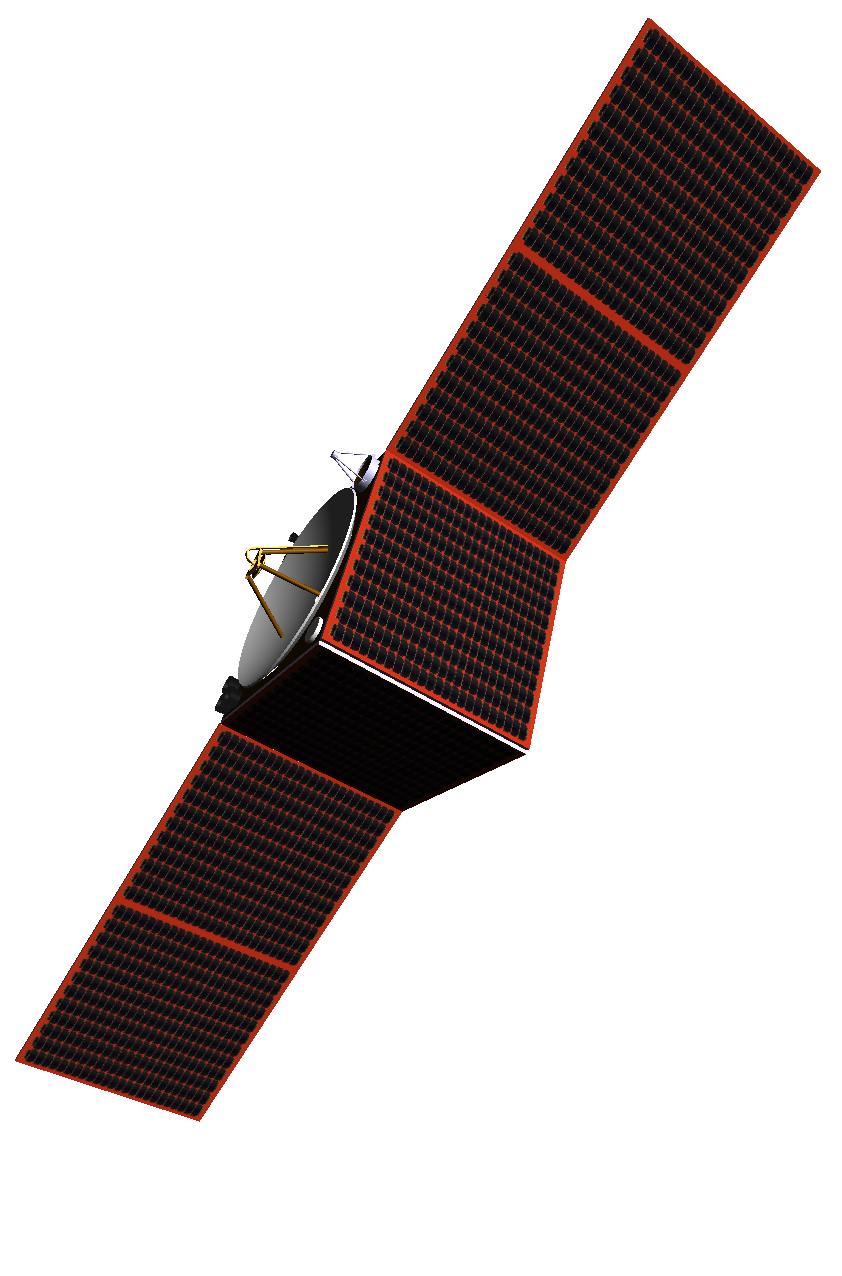
\includegraphics[angle=-90,width=\textwidth]{Images/bw1_bild2.png}
  \end{center}
  \caption{\BW}
  \label{fig:Spacecraft-BW-1}
\end{figure}

\BW\ will be propelled by a combination of Pulsed Plasma Thrusters (PPTs), developed at IRS by \textcite{Nawaz2008} and a thermal arcjet similarly developed at IRS by \textcite{Bock2007}. Performance parameters for these thrusters based on laboratory tests are listed in \autoref{tab:BW1-performance}. The thrusters will be arranged as seen in \autoref{fig:Thrust-vectoring}, with an arcjet surrounded by four PPTs. This arrangement was recommended to allow reaction wheel desaturation in pitch and yaw; the deflector plate was a conceptual idea to allow roll desaturation. The author declines to comment on the efficacy of this mechanism, as it is well outside the scope of this project.

\begin{table} [h]
  \caption{Performance parameters of \BW\ thrusters}
  \label{tab:BW1-performance}
  \begin{center}
    \begin{tabular} {cccc}\toprule
      Propulsion system & Arcjet & PPT \\\midrule
      Number of active units & 1 & 4 \\
      Power required per unit (W) & 801 & 52\\
      Thrust produced per unit (mN) & 102.5 & 1.22\\
      Exhaust velocity (ms$^{-1}$) & 4768 & 27000\\\bottomrule
%      Specific impulse (s) & 486 & 2753\\\bottomrule
    \end{tabular}
  \end{center}
\end{table}

\begin{figure} [h]
  \begin{center}
    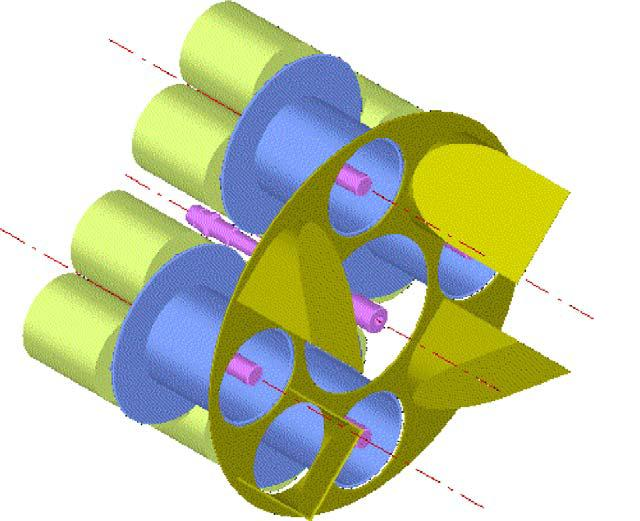
\includegraphics[scale=0.25]{Images/thrust-vectoring.JPG}
  \end{center}
  \caption{Arrangement of arcjet (centre) and 4 PPTs on \BW, with a conceptual mechanism allowing for thrust vectoring. Image used courtesy of \textcite{Roeser2006}.}
  \label{fig:Thrust-vectoring}
\end{figure}

Due to the design decision to fix both the solar panels and the thrusters with respect to the body, the spacecraft will have to alternate between thrusting along the desired vector with reduced power generation, and coasting in order to orient the solar panels towards the sun. Consequently on-board power storage is required.

The \BW\ mission architecture has been broken down into the following seven phases, as published by \textcite{web_BW-1}:
\begin{enumerate}
  \item Launch Phase: the spacecraft is delivered into Geosynchronous Transfer Orbit (GTO).
  \item Ascent Phase: the spacecraft's orbit is extended above the van Allen belt using the arcjet.
  \item Cruise Phase: Orbit extension up to lunar gravitational sphere of influence using PPTs.
  \item Capture Phase: Insertion into highly elliptical lunar orbit using the arcjet.
  \item Descent Phase: Transfer of the satellite into a high inclined, circular orbit (approximately 100~km altitude) using PPTs.
  \item Science Phase: Remote sensing of the surface of the Moon (stable orbit requiring minimal stationkeeping; however energy requirements are increased by scientific instruments and data transfer).
  \item Impact Phase: Controlled impact of the satellite onto the lunar surface using the arcject.
\end{enumerate}
Phase one is expected to be provided by a commercial launch vehicle such as the Indian Space Research Organisation (ISRO)'s Geosynchronous Satellite Launch Vehicle (GSLV), seen in \autoref{fig:GSLV}, which launches from Sriharikota. Phase two, concerning ascent from GTO to an orbit above the van Allen belts, has undergone preliminary analysis by \textcite{Letterio_thesis}. Phase four has undergone preliminary study by \textcite{Moellman2005}, while the specifications for the lunar orbit (phase six) have been developed by \textcite{Zeile2010}. Various impact scenarios have been developed by \textcite{Trawny2004}. The research presented in this thesis brings these preliminary studies together, including more detailed and accurate constraints, and examines the interdependencies between phases 2 to 5.

\begin{figure} [h]
  \begin{center}
    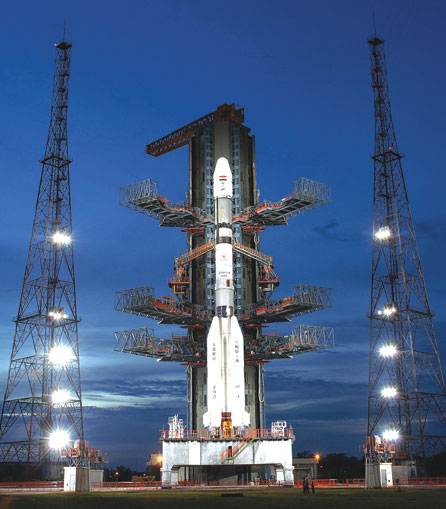
\includegraphics[scale=0.50]{Images/GSLV2.jpg}
  \end{center}
  \caption{Indian Geosynchronous Satellite Launch Vehicle. Image used courtesy of ISRO.}
  \label{fig:GSLV}
\end{figure}